%!TEX root = ../thesis.tex
%*******************************************************************************
%****************************** Second Chapter *********************************
%*******************************************************************************

\chapter{APIs in the Public Sector}

\ifpdf
    \graphicspath{{Chapter2/Figs/Raster/}{Chapter2/Figs/PDF/}{Chapter2/Figs/}}
\else
    \graphicspath{{Chapter2/Figs/Vector/}{Chapter2/Figs/}}
\fi

Modern technology in combination with the Internet have permitted people
to carry out online most of their daily activities and their transactions.
These widespread and rapidly expanding possibilities have increased citizens'
and business expectations in their interactions with government.

People are demanding transparency, accountability, access to information and
competent service delivery from their governments. They also expect policies
and services to be tailored to their needs and address their concerns.

In this section, we will analyze how APIs are used in the public sector.
At first we will delve into APIs common uses, such as creators of ecosystems
or as means to facilitate integration solutions.
Specific examples are described in order to elaborate on APIs use in the public
sector.Moreover, we will
cover some challenges and considerations as well as examine data on the APIs
advertised in one of the most respected API Directories such as
ProgrammableWeb as a further indicator of the way APIs are used in the
public sector.


Common uses of APIs concern their capacity as creators of ecosystems
in the public sectors. Specific examples prove this aspect.


\section{APIs as a mean to create ‘ecosystems’ in the public sector}

API based ecosystems can be described as the extended interrelationships enabled
by developers who build applications that connect various groups of stakeholders
to each other via API based solutions that use the internet to communicate~\citep{api_ecosystems}.

An ecosystem may be created within a government entity, between entities or
it may be wider reaching, for example between two governments or between a government,its citizens and third party providers.

\begin{figure}
\usetikzlibrary{arrows,positioning}

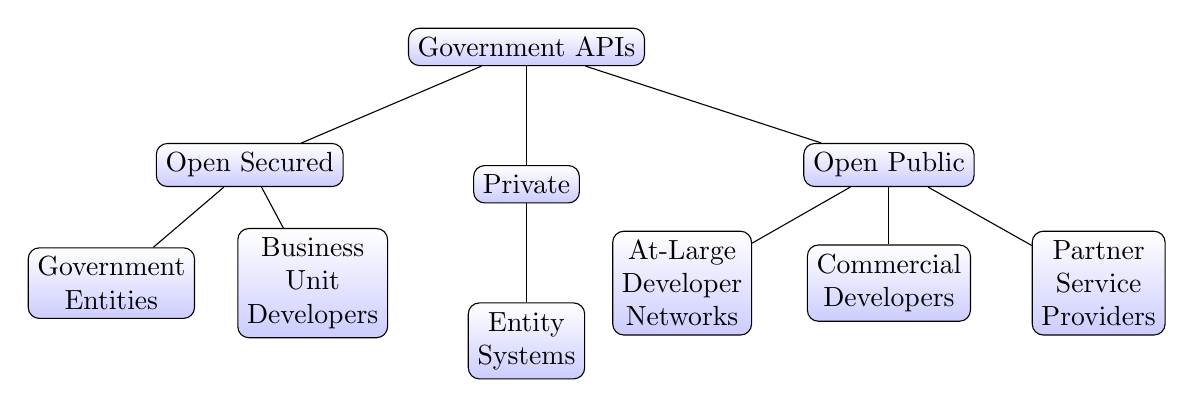
\begin{tikzpicture}[sibling distance=10em,
every node/.style = {shape=rectangle, rounded corners,
	draw, align=center,
	top color=white, bottom color=blue!20}]]
\node {Government APIs}
child { node {Open Secured}
	child { node {Government \\ Entities}}
	child { node [anchor=east] {Business \\ Unit \\ Developers} } }
child { node [anchor=north] {Private}
	child { node [anchor=north] {Entity \\ Systems}} }
child { node [anchor=west] {Open Public}
	child { node [anchor=west] {At-Large \\ Developer \\ Networks}}
	child { node {Commercial \\ Developers} }
	child { node [anchor=east] {Partner \\ Service \\ Providers} } };
\end{tikzpicture}

\label{Figure 1}
\caption{Ecosystems enabled by government APIs}~\citep{proactive_api}
\end{figure}


The figure above illustrates the way in which APIs are used as well as the typical
ecosystem that they facilitate in the public sector.
\begin{itemize}
	\item \textbf{Private – Entity Systems}: These APIs are generally used to facilitate
	 the sharing of data between systems within an entity, avoiding the need
	 for complex point to point integration. Outside of the entity they are not visible
	 to any person or body and are generally in the domain of the IT
	 department. An example maybe a link between an internal Administration system and a Payroll solution.
	 \item \textbf{Open Public – At Large Developer Networks}: Open APIs (i.e. they do
	 not require permission to access them) are the entry point for developers
	 to access large public data sources such as a census information or other
	 similar statistical data, perhaps live sensor data from which to create
	 citizen-facing applications.
	 \item \textbf{Open Public – Commercial Developers}: Similarly to Open Public,
	 but developers who are
	 looking to gather openly available data for use, usually, in applications
	 that can be sold. They may add value by combining the data, i.e.
	 data on public transportation networks with location data available on an
	 individual’s smartphone to help the citizen make travel choices in real-time.
	 Due to this open access, third-party integration of software is not only easier
	 but also less problematic. Developers have access to the API at all times, so they can ensure that the two-way communication between assorted pieces of software is accurate.
	 
	 It is also worth noting the economic stimulation that this can bring. Transport
	 for London’s policy of working with major IT players (Google, Apple, Waze etc.)
	 but allowing their data to be available via the Open Government License has led
	 to the creation of additional economic activity in the order of £100m of direct
	 value and has enabled some 1,000 jobs~\citep{api_industrial_data}.
	 \item \textbf{Open Public/Secured – Partner Service Providers}: The APIs are open to
	 partners often in the private sector which may include healthcare providers
	 for example, who in some member states are interested in sharing healthcare
	 records or confirming eligibility for free or subsidized treatment based on
	 data held by a government organization.
	 \item \textbf{Open Secured – Government Entities}: These APIs are available to other
	 government organizations and allow them to share data only after they have
	 authenticated. This supports many of the core tenets of digital government,
	 allowing agencies to gather data on a citizen only once, and then share it
	 securely. For instance this may involve the sharing of citizen data between
	 the agency responsible for income and taxation, and those providing benefits in
	 order that eligibility could be confirmed. Estonia X-Road and Amsterdam City
	 Data are some examples of this.
	 
	 Besides not being specifically mentioned in the diagram above, the ability to use
	 APIs is not constrained by sector or geographical boundaries. Open Secured
	 – Government Entities could include an application to application link
	 between governments of different member states. A good example would be the Estonian X-Road Platform which uses APIs to
	 share citizen’s healthcare information with Finland.
	 
	 \item \textbf{Open Secured – Business Unit Developers}: Similar to the above, but instead of basic inter-entity data sharing, in this case the data is being
	 consumed and then in some way supplemented in order to be useful by developers
	 within a government entity. They are used to create custom applications around
	 internal data assets for entity use.
\end{itemize}

In summary, the creation of an ‘ecosystem’ of providers and consumers fosters
openness and efficiency and can also spawn the development of innovative service
models, some of which may lead to revenue generation for the entities concerned
(i.e mapping data~\citep{os_places}, or gazetteer data). The ability of APIs to provide access
into the governments major operations and data, in turn allows it to realize its objectives
of openness, and of delivering efficient, secure, transparent and interoperable
citizen centric services. The APIs are, therefore, a significant technological
component, which will support the evolution of public service delivery
models, enabling entities to accelerate their shift from eGovernment to
Digital Government.

\section{APIs as a mean to overcome complex integration}

Many EU countries have built their computing infrastructure over the course of
many years, constructing large, complex information systems featuring
interfaces to share information from one system to another. Most of these
interfaces were point to point and tailored to the needs of a particular
project or entity at a given time. As the number of interfaces increased, so did the
maintenance burden; the inter-relationships and the data duplication leading to an
costly, complex and inefficient architecture~\citep{deloitte_insights}. In summary, these
legacy government systems and associated business processes increase
risk and exacerbate challenges in data sharing and service delivery across the
ecosystem.

APIs provide an opportunity, in other words a structural solution, to permit the
information within these legacy systems to be exposed with relatively low complexity
and investment. They can be connected to legacy systems of record such as ERP
systems~\citep{erp_integration}, or citizen records to make the data records directly available
helping in this way to bypass the complex interfaces of already existing systems,
and allow data sharing to be accomplished more easily. This implies that a
well-designed government ecosystem could so that citizens or businesses will have to
provide the same information less frequently (Once Only Principle, OOP).

A characteristic EU example of where API infrastructure is currently being used to overcome
the limitations of traditional integration solutions is Estonia’s X-Road Platform.
It allows citizens to provide ordinary ‘private and sensitive’ data to public administrations only once, for instance, place of residence or place of birth. The ecosystem also includes
private institutions such as banks who can have access in order to perform various
functions.

\textbf{ESTONIA X-ROADS PLATFORM}

“X-Road is the backbone of e-Estonia. Invisible yet crucial, it allows the
nation’s various public and private sector e-Service databases to link up and
function in harmony.”~\citep{x-road}

X-Road is a government API framework developed by the Estonian Government
and licensed under the MIT license. It is also used as a backbone of the Finnish
National Data Exchange Layer.Initially built for SOAP/XML web services, it now
extends to REST APIs. Rather than requiring governments to develop API management
directly, X-Road provides an API management layer, including an API gateway,
which is open-sourced and available to governments worldwide.~\citep{gov_transformation}

The X-Road solution includes a security server to provide authorization
for government API access. It also provides central monitoring of
API traffic.Apart from the management of APIs, it also provides an
aggregation layer in front of multiple databases. This makes easier the creation
and delivery of data access APIs.

Since each government service/entity has its own databases they all use X-Road
to securely communicate and share ‘private and sensitive’ data to protect the
‘once only’ principle of sharing data with government. The service also incorporates
many other sectors numbering over 900 organizations and enterprises including those
in the banking, health and utility sectors~\cite{x-road}. Whilst they may use the platform to
perform functions such as identity verification, powerful use cases such as automated extraction of funds from bank accounts for those failing to keep up to date with
taxes are possible.

Given the above, the X-Road itself is a ‘very low level engineered application’
according to Andrew Kütt ~\citep{andrew_kutt}. Following certification, an organization
deploys an x-road gateway
so that it can hold secure private communications via APIs with other certified
organizations that are legally able to share data with it. As a collective set 
of tools, the e-Estonia services provide the government of Estonia and its partners,
including Finland, with a platform on which to innovate and use digital
transformation to deliver new services across the globe.

\section{APIs support open government initiatives}

Open Government is the opening up of government processes,
proceedings, documents and data for public scrutiny and involvement and is
now considered as a integral element of a democratic society~\citep{open_gov}.
The Open government initiative started in 2009 by Barak Obama~\citep{whitehouse_archives}, after that,
a great number of governments embraced open data initiatives. This is based on the
belief that greater transparency and public participation can both lead
to better policies and services, and also promote public sector
integrity, which is necessary to regaining the trust of citizens in the
neutrality and reliability of public administrations.

It has been acknowledged that APIs faciltate the opening of huge data sources
to citizens and other third parties. The Open Government imperatives have meant
that API technology has been exploited outside of the ‘IT department’,
providing access into large open data stores so that developers and their
applications and websites can more easily use it. When a government agency
publishes an API for their data set, they open up new and innovative ways to
access the data. A developer might develop a mobile or web app to display the
data as it is or allow simple queries or automatically depicted in charts.

The most relevant public sector that expose government datasets is The European
Data Portal~\citep{edp_use_cases} (EDP).

\textbf{European Data Portal (EDP)}

The EDP provides access to 79 different catalogues, most with tens of thousands of
open datasets provided by various member state governments. The same site also provides
access to over 300 use cases (services or applications) that have been developed
using the open data sets available. Some of these applications have been created
using APIs to query the EDP.

The access to the Portal is provided by a machine-readable API which enables its
users to search, create, modify and delete metadata on the portal.~\citep{edp_data_portal} APIs are
available both via the Comprehensive Knowledge Archive Network (CKAN)~\citep{edp_api_v3} and
SPARQL~\citep{edp_sparql} endpoints.

\section{APIs as a mean for innovation}

APIs enable new innovative service models which better engage citizens and allow
for more efficient delivery of their services. These services no longer have to
be provided directly by the agency, partners and citizen developers can use
available data to enable new solutions. Smart Cities and the vast amount of data
produced by sensors supports the development of dynamic platforms and ecosystems
providing contextualized, real-time location-based data from IoT or crowdsourcing
to business partners and startups giving them opportunities to create new services
or improve existing ones.

Transport for London is a successful platform which uses APIs in an innovative way to deliver services.

\textbf{TRANSPORT FOR LONDON (TfL)}

At a recent European conference~\citep{api_industrial_data}, Transport for London detailed the investment that they had made:
\begin{itemize}
	\item 200 data elements are made available through an API to about 12,000
	developers producing over 600 apps that almost 40\% of Londoners use.
	
	\item TfL has formed partnerships with major IT players such as Apple
	(for mobile payment, rental of bikes), Twitter (for pushing alerts out),
	a two-way data-sharing agreement with Waze (enriching the app with data
	from the road network that TfL manages while benefiting from data collected
	through Waze) and Google (enriching the maps application with real-time data).
	
	\item The data can be consumed under the terms of the UK Open Government
	License with some minimal additions for free. This is done under a statutory
	requirement as part of UK legislation. Mechanisms are in place to ensure that
	consumption remains at an acceptable level. There is one single set of data
	at the base that are both consumed by TfL for its purposes and by third	party
	developers. Developers must give attribution to TfL for the fact that their
	app includes TfL data.
	
	\item In terms of creation of additional economic activity, it has been
	estimated that this policy	generates GBP 100m of direct value and has created
	over 1,000 jobs.
	
	\item All data made available is data that TfL collects anyway for its own
	purposes. TfL is not collecting additional data just to make it available to
	third parties.
	
	\item Combining data provided by TfL with privately-held data can bring additional innovative ideas (e.g. "Are	there correlations between rainfall and collisions involving cyclists?”).
\end{itemize}

\section{Challenges and Considerations}

To a great extent, externally facing public sector APIs involve the movement
of data that is sensitive as it usually refers to information regarding
a citizen. This creates a number of consistent challenges for government:
\begin{itemize}
	\item \textbf{Regulation} – APIs play an important role in the facilitation of
	government transparency. A recent EU ruling~\citep{eu_funding} makes providing
	transparency into all IT services that will be used in technology projects
	a requirement in order to receive government funding. APIs are bound to support the
	technology required for the transparency principle.
	
	\item \textbf{Further regulatory considerations} - Considerations which
	must be adhered to when	exposing data through any type of interface are
	the General Data Privacy Regulation~\cite{eu_gdpr} (GDPR), the Payment
	Services Directive	(PSD2)~\citep{eu_payment_directives} and the Public Sector Information
	Directive (PSI)~\citep{public_sector_info}.
	
	\item \textbf{Security} – APIs share data, services, and transactions in order to create new services. This inherently increases the permeability of an
	organization’s network, which can expose new vulnerabilities for
	exploitation. For that reason, APIs must be properly protected to ensure data
	privacy as well as citizen confidence in terms of service delivery.
	APIs meant for access to public data should be secured from inappropriate
	use or abuse such as denial of service. A number of potential security solutions exist.
	For example the Greek Government API of the Digital Solemn Declaration/ Authorization
	application uses solutions such as OAuth 2.0 along with OpenId Connect. Other solutions
	include Certificate based authentication, which are used in conjunction with a wider cyber security strategy and cryptography.

	
	\item \textbf{Specifications or Standards} - Standards for APIs are available in
	clusters such as the OGC~\citep{open_geospatial_consortium} standard, and the developing ISO
	standard in Financial Services~\cite{iso}. However, most organizations are
	developing APIs based on an internally accepted specification or style guide
	to ensure consistency, rather than what might normally be recognized as
	a de facto ‘standard’. Every API comes with detailed documentation for
	consumers which	specifies the type of API	(RESTful, GRAPHQL,
	GRPC etc.). There is little intention for further standard
	development in the aftermath of ‘Open Government’~\citep{interface_standardisation}.
\end{itemize}

FIWARE Foundation (Future Internet Ware) attempts to
overcome some of the challenges mentioned above. It is funded by
the EU, corporate membership and venture capital funding and has
created a scalable open source platform in order to access and manage heterogeneous context information through
open APIs~\citep{eu_innovation_programmes}. A standard for exchange of context information: FIWARE-NGSI
(Next Generation Service Interface) is an open standard API to be used for Smart
Cities, Smart Industry and Smart Agrifood as mentioned by Ulrich Ahle, CEO FIWARE. FIWARE success
has been acknowledged by the EU, however a standardized API that is universally used has not been defined.
\begin{itemize}
	\item \textbf{Business Models} – The government does not usually charge for data that is publicly owned and it is used for the public good thus not generating much income by users
	who wish to use that data. Examples of charging mechanisms being in place
	are	limited, one being the UK’s Ordnance Survey maps~\citep{os_places}, and KLIP.
\end{itemize}

\section{Quantitative assessment of API use in the public sector}

It is not easy to reliably quantify the amount of public sector organizations
that are currently using APIs internally, but the total number it is estimated to amount to millions~\citep{deloitte_insights}. Organizations
that create externally facing APIs in order to interact with huge data sources
are common worldwide which is obvious by the numbers of APIs registered with online API Directories i.e ProgrammableWeb ~\citep{programmableweb_apis}. To lure the maximum amount of developers to leverage the
data being exposed, organizations publish their API with high-level
technical specification. For that reason, an analysis of a popular
directory is likely provide indicative information concerning the number of EU
public sector APIs as well as the sectors and associated public services that they support.

The best known and globally recognized API directory is ProgrammableWeb~\citep{programmableweb_search}.
Nordic APIs~\citep{nordic_apis} comments that it is ‘exhaustive’ and ‘comprehensive’ and is
both hand curated and searchable. 

From almost 23,000 listed APIs in ProgrammableWeb (as at December 2019),
we selected the ‘Government’ category which reduced the number searched to 787
(including the deprecated ones).
According to our findings only 110 of the 787
Government category APIs advertised on the directory originated from the EU.
This could be explained by the fact that ProgrammableWeb is based in the United States
and not in Europe. As we can see in the table below most APIs were developed at a National level.

% Note: It may be necessary to compile the document several times to get a multi-page table to line up properly
\begin{longtable}[c]{|l|l|l|}
	\hline
	\multicolumn{1}{|c|}{\textbf{Scale (EU Coutries)}} & \multicolumn{1}{c|}{\textbf{APIs}} & \multicolumn{1}{c|}{\textbf{Number of APIs}} \\ \hline
	\endfirsthead
	%
	\endhead
	%
	City & \begin{tabular}[c]{@{}l@{}}- Transport for London\\ - City of Helsinki Service Mapping\end{tabular} & 12 \\ \hline
	Regional & \begin{tabular}[c]{@{}l@{}}- The Statistical Institute of Catalonia\\ - Open Greater Manchester\end{tabular} & 7 \\ \hline
	National & \begin{tabular}[c]{@{}l@{}}- Denmark Central Business Register (CVR)\\ - Where Does My Money Go (UK budget\\ spend)\end{tabular} & 71 \\ \hline
	International & \begin{tabular}[c]{@{}l@{}}- Openspending\\ - World Government Data\end{tabular} & 7 \\ \hline
	EU & \begin{tabular}[c]{@{}l@{}}- Open Patent Services\\ - VAT\\ - OrganiCity Permissions\\ - It's Your Parliament EU Data\\ - Nephics European VAT Number Validation\\ - iTranslate4.eu\\ - European Union Legislation\end{tabular} & 12 \\ \hline
	\caption{ProgrammableWeb EU API Analysis}
	\label{PWAnalysis}
\end{longtable}

The majority of these APIs provide access to open data sources for developers to use in
order to create applications for commercial use while others focus more on citizens and democracy.


\section{Summary}

APIs expose data in a very cost effective way through both private and public
ecosystems, which developers can consume  to generate benefits for citizens, business
and for the economy. The amount of APIs is growing rapidly each year as illustrated in 
online API Archives. This proves the value that they add for the public sector across a
variety of use cases.
